\maketitle{}
\section{ Using Angular CLI in an Nx Workspace }

Now that we have created an nx workspace, let's create our app. Run
\begin{verbatim}
  ng g app angularPixelIllustrator --routing
\end{verbatim}

This will create an app called angular-pixel-illustrator\footnote{that's right
angular cli will automatically convert camel case to dash case} with routing
capabilities using the Angular CLI \footnote{If you will recall, we discussed
the Angular CLI folder/file directory in the Angular CLI Chapter}.

We can now serve\footnote{I.e. run on a server for development reasons} our app,
by running:
\begin{verbatim}
  ng serve
\end{verbatim} \footnote{It's important to note, that ng serve will open up
angularPixelIllustrator by default. As we begin to add more apps, it will make
more sense to specify specific app being opened.}


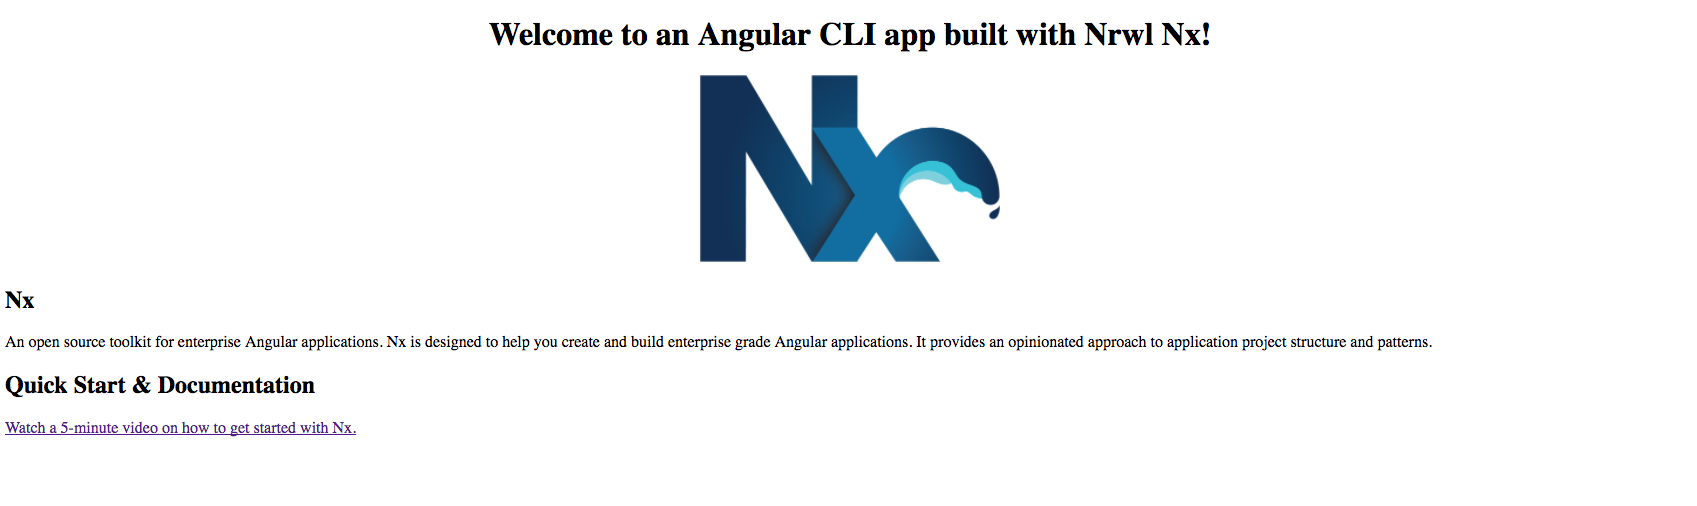
\includegraphics[width=13cm, height=9cm]{angular-cli-post-nx/angular_nx_initial_screen}

At this time, if you were to go to localhost:8080 you will see our app, is
ready to go.

Let's now create our first component. For our Pixel Illustrator, we want a form.
We will name the component chooseSize.

\subsection {Wait a Minute!}
Before we go ahead and create our component, we are going to want to tidy up
our folder architecture. The architecture we are introducing in this book is
heavily influenced by two projects. One, Nrwl, and by extension Nx. The other is
the example app, introduced in the ngrx/platform repo \footnote{It can be seen
here: https://github.com/ngrx/platform/tree/master/example-app}.

\subsubsection {Sidebar}
At the time of thiwriting there is one main area of conflict with regards to
ngrx/store v. Nx. Even though we have not experienced it yet, it makes sense to
talk about it before moving on from the cli/nx workspace chapters. Nx is very
opiniated with regards to it's folder structure. It believes everything should
be turned into it's own module, and all files related to that module should
be encapsulated inside of it. This includes (and if you are not familiar, do not
worry, we will get to it in later chaptes ) pipes, services, interfaces, guards,
and enums.

In the ngrx/example-app project, these will be split into separate folders, and
the appropriate file, will be put into that specific folder. I would imagine
that many on the ngrx/platform team agrees with nrwl/nx. I most certainly do,
and especially with state management, it makes sense for all others items to
be encapsulated into their appropiate folder. If it is something that should be
shared across app, then it should be put into it's own library. Something that
we will discuss moving forward.

\subsection {Phew, sidebar over, moving on}

In order to create our component we run the following angular cli command:

\begin{verbatim}
  ng g component chooseSize
\end{verbatim}
